\clearpage
\chapter{Overview of the Game of Monopoly}\label{chap:monopoly}

Monopoly is a game where players traverse a path around a board on which most
spaces represent a property which players can buy (See
Figure~\ref{figure-monoboard}). Other players must pay ``rent'' to the owner of
a property when they land on that property.

\begin{figure}[htp]
\centerline{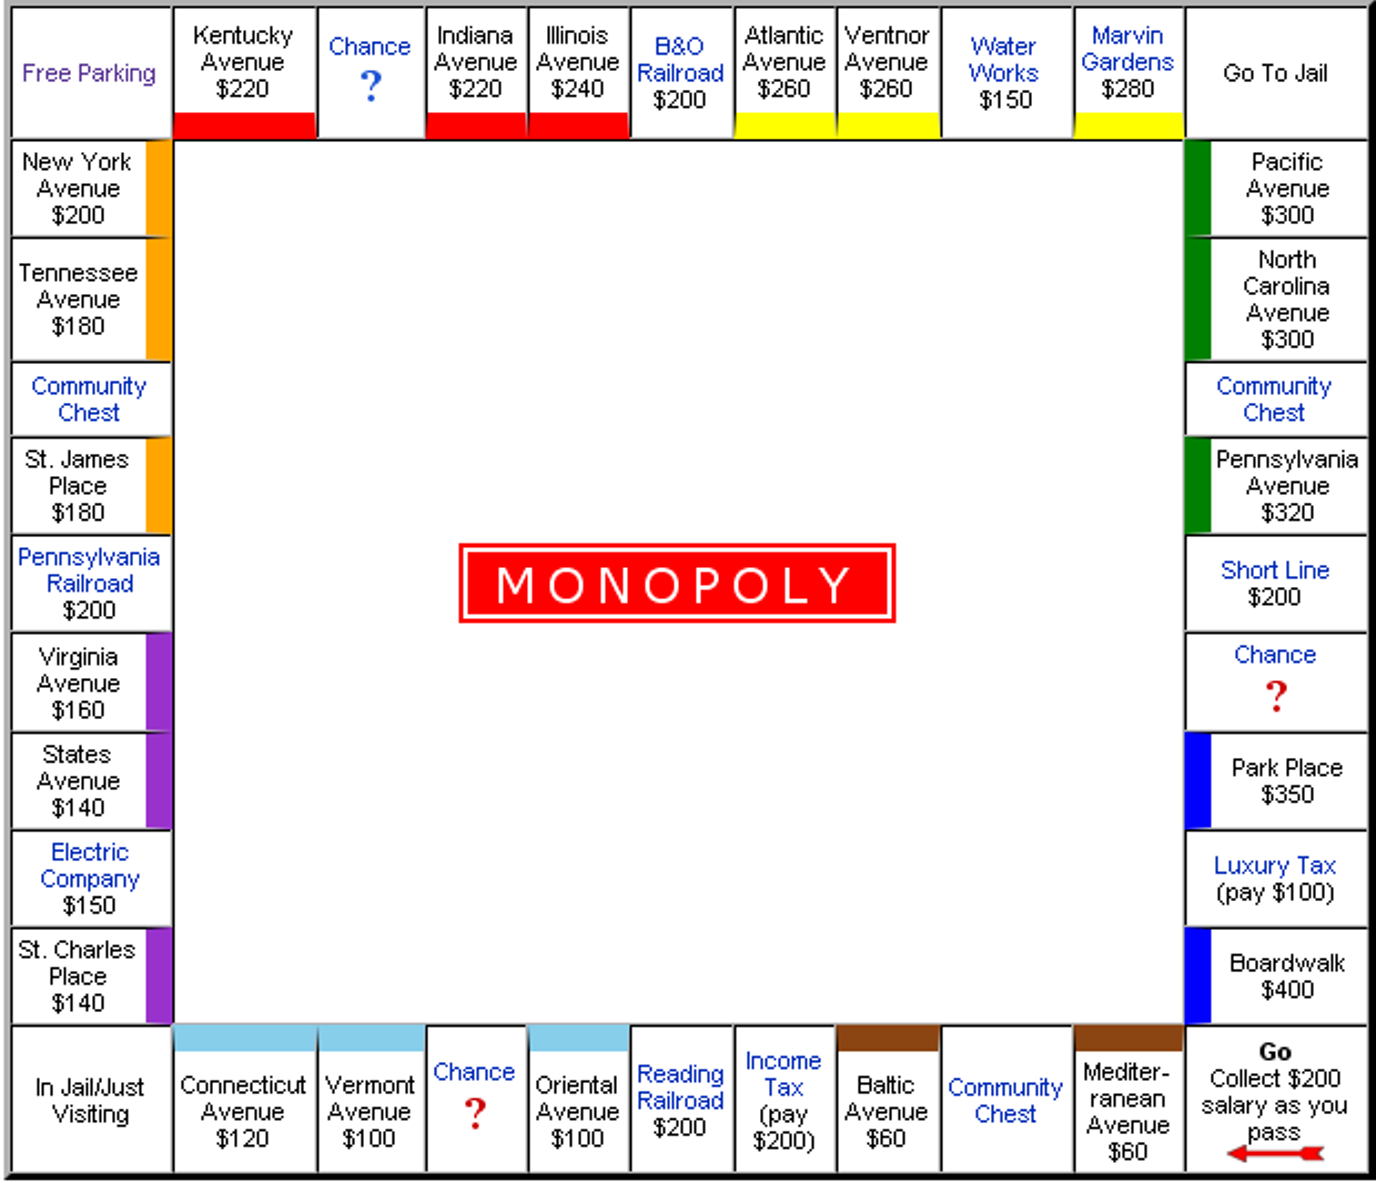
\includegraphics[width=1.0\columnwidth]{Figures/Monopoly.png}}
\caption[Board layout for Monopoly]{The board layout for Monopoly. For this
study, the edge of the board containing ``Go'' through ``Connecticut Avenue'' is
south. Proceeding clockwise, the next edge is west. The top of the figure is
north. The final edge of the board is east. South includes the cheapest
properties; east contains the most expensive. Monte Carlo simulations of dice
rolls show that the locations that are most landed on are on the west and north
edges of the board.}
\label{figure-monoboard}
\end{figure}

When one player owns all the properties in a color group (a monopoly), the
player can ``develop'' the properties by building houses or hotels. This
increases the rent value which increases the probability that an opponent will
not be able to pay the rent. If a player cannot pay rent, the player must sell
or mortgage properties, and if that is not possible, give their properties to
the owner. The winner is the player who bankrupts the other players.

Another important feature of Monopoly is the ability of players to trade
different properties. Because of the random nature of a player's moves, it is
improbable that a single player will be able to land on and buy all the
properties in a group. So, players usually must trade with other players to gain
a monopoly on a property group.

\section{Movement}
Players take turns moving around the game board based on the roll of two dice.
Thus, for each move, the player will move between 2 and 12 spaces. The player's
location on the board is represented by a token.

If a player rolls doubles (the two dice have the same value), the player is
allowed a second roll of the dice. If the player rolls doubles on the second
roll, the player is allowed a third roll. If the player rolls doubles a third
time, they must move their token directly to Jail.

\section{Game locations}
There are 28 locations on the game board that can be bought by the players. The
locations are divided into 22 streets, which are further grouped into 8 color
groups, 4 railroads, and 2 utilities. Figure~\ref{figure-street} shows the
property card for a street location.

\begin{figure}[htp]
\centerline{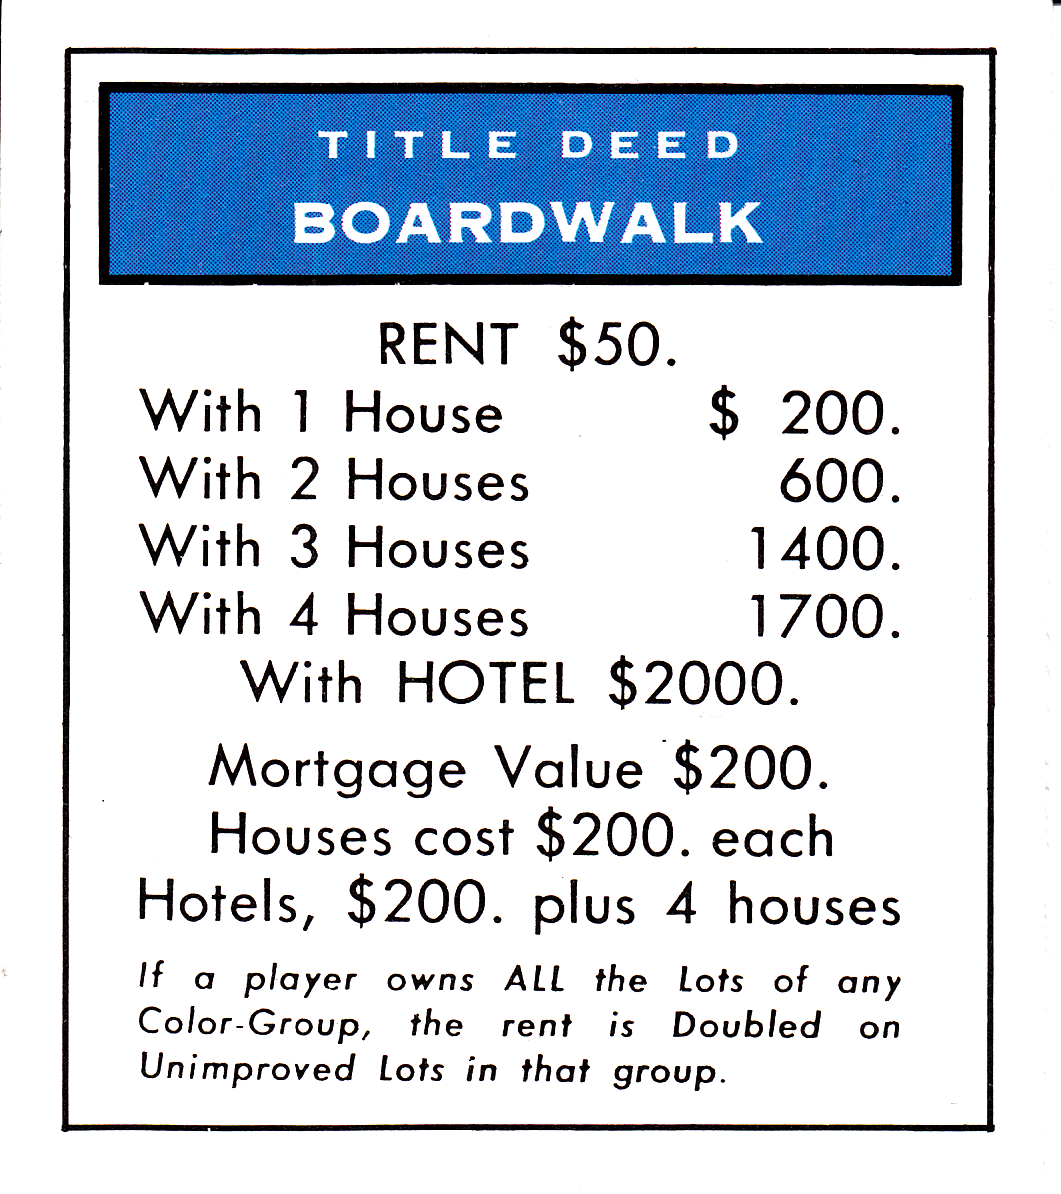
\includegraphics[width=0.5\columnwidth]{Figures/Boardwalk.png}}
\caption[Example property card]{The property card for the street location
Boardwalk. The card lists various costs including how much rent an opponent
pays, the mortgage value of the property, and how much the owner pays to buy
houses or a hotel.}
\label{figure-street}
\end{figure}

If the player lands on an unowned location, the player may buy the property. If
the player declines to buy the property, the property is auctioned among all
players (including the player who originally declined to buy the property).
If the player lands on a property that is already owned, the player must pay
rent to the owning player.

The other 12 locations on the board cannot be owned by any player. For this
study, only one of those locations is important. That location is the corner
space marked ``Jail.'' There are three circumstances that can send a player to
Jail: drawing a special card marked ``Go To Jail,'' landing on the corner marked
``Go To Jail,'' or rolling doubles three times in a row in one turn.

A player whose token is in Jail may, on their next turn, pay \$50 and leave jail
(after rolling the dice), or may choose to attempt to roll doubles to leave
jail. If the player fails to leave jail on three consecutive turns, they must
immediately pay \$50 and move the number of spaces shown on the dice.

Six locations on the board are special locations. These are the locations
labelled Chance or Community Chest. They require the player to draw a card and
take the action directed by the card, such as paying or receiving money, or
advancing to a specific location. This is another source of randomness in the
game since the card that a player receives is random.

\section{Game Strategies} \label{m_gamestrategies}
Over the years since the game was invented, players have built up a set of rules
of thumb for successfully playing the game. Some of those strategies are as
follows.

\begin{itemize}
  \item {Buy a property if no other player owns a property in its color group.}
  \item {Buy a property if it gives you a second or third property of its
  group.}
  \item {Buy a property if it blocks an opponent from controlling a color
  group.}
  \item {Buy a property if it is an orange property (always block this group if
  you can).}
  \item {Pay \$50 and get out of Jail early in the game while many Monopoly
  properties remain unowned and undeveloped.}
  \item {When most Monopoly properties are developed between Jail and the Go to
  Jail space, roll the dice and hope to stay in Jail.}
\end{itemize}